\ifdefined\maindoc\else
% typesetting this chapter as a standalone document
\def\doctitle{Skinning}
% starting definitions for both the main document and stand-alone chapters
\documentclass{book}

\def\mech{artisynth.core.mechmodels}
\def\mgeo{maspack.geometry}

% Add search paths for input files
\makeatletter
\def\input@path{{../}{../../}{../texinputs/}}
\makeatother

\usepackage{amsmath}
\usepackage{framed}
%%
%% Default settings for artisynth
%%
\NeedsTeXFormat{LaTeX2e}
%%\ProvidesPackage{artisynthDoc}[2012/04/05]

\usepackage[T1]{fontenc}
\usepackage[latin1]{inputenc}
\usepackage{listings}
\usepackage{makeidx}
\usepackage{latexml}
\usepackage{graphicx}
\usepackage{framed}
\usepackage{booktabs}
\usepackage{color}

\newcommand{\pubdate}{\today}
\newcommand{\setpubdate}[1]{\renewcommand{\pubdate}{#1}}
\newcommand{\code}[1]{{\tt #1}}

\iflatexml
\usepackage{hyperref}
\setlength\parindent{0pt} 
\else
%% then we are making a PDF, so include things that LaTeXML can't handle: 
%% docbook style, \RaggedRight
\usepackage{ifxetex}
\usepackage{xstring}
\usepackage{pslatex} % fixes fonts; in particular sets a better-fitting \tt font

\usepackage[most]{tcolorbox}
\definecolor{shadecolor}{rgb}{0.95,0.95,0.95}
\tcbset{
    frame code={}
    center title,
    left=0pt,
    right=0pt,
    top=0pt,
    bottom=0pt,
    colback=shadecolor,
    colframe=white,
    width=\dimexpr\textwidth\relax,
    enlarge left by=0mm,
    boxsep=0pt,
    arc=0pt,outer arc=0pt,
}%

\usepackage[A4]{artisynth_papersize}
%\usepackage[letter]{artisynth_papersize}
\usepackage[hyperlink]{asciidoc-dblatex} 

%\usepackage{verbatim}
\usepackage{ragged2e}
\setlength{\RaggedRightRightskip}{0pt plus 4em}
\RaggedRight
\renewcommand{\DBKpubdate}{\pubdate}
\renewcommand{\DBKreleaseinfo}{}
\fi

% set hypertext links to be dark blue:
\definecolor{darkblue}{rgb}{0,0,0.8}
\definecolor{sidebar}{rgb}{0.5,0.5,0.7}
\hypersetup{colorlinks=true,urlcolor=darkblue,linkcolor=darkblue,breaklinks=true}

%%%%%%%%%%%%%%%%%%%%%%%%%%%%%%%%%%%%%%%%%%%%%%%%%%%%%%%%%%%%%%%%%%%%%%%%%%%%%
%
% Define macros for handling javadoc class and method references
%
%%%%%%%%%%%%%%%%%%%%%%%%%%%%%%%%%%%%%%%%%%%%%%%%%%%%%%%%%%%%%%%%%%%%%%%%%%%%%
\makeatletter

% macro to enable line break if inside a PDF file
\def\pdfbreak{\iflatexml\else\\\fi}

% code inspired by http://stackoverflow.com/questions/2457780/latex-apply-an-operation-to-every-character-in-a-string
\def\removeargs #1{\doremoveargs#1$\wholeString\unskip}
\def\doremoveargs#1#2\wholeString{\if#1$%
\else\if#1({()}\else{#1}\taketherest#2\fi\fi}
\def\taketherest#1\fi
{\fi \doremoveargs#1\wholeString}

% Note: still doesn't work properly when called on macro output ...
% i.e., \dottoslash{\concatnames{model}{base}{foo}} fails 
\def\dottoslash #1{\dodottoslash#1$\wholeString\unskip}
\def\dodottoslash#1#2\wholeString{\if#1$%
\else\if#1.{/}\else{#1}\fi\dottaketherest#2\fi}
\def\dottaketherest#1\fi{\fi \dodottoslash#1\wholeString}

\def\hashtodot #1{\dohashtodot#1$\wholeString\unskip}
\def\dohashtodot#1#2\wholeString{\if#1$X%
\else\if#1\#{.}\else{#1}\fi\hashtaketherest#2\fi}
\def\hashtaketherest#1\fi{\fi \dohashtodot#1\wholeString}

%\dollartodot{#1} does the same thing as \StrSubstitute[0]{#1}{\$}{.}
% from the packahe xstring. We define \dollartodot instead because
% LaTeXML does not implement xstring.
%
% Note that for the substituion to work, we need \ifx instead of \if,
% since otherwise escaped characters won't work properly:
% if #1 = \$, then \if#1* seems to compare '\' and '$' (and output '*'),
% rather than comparing '$' to '*'
\def\dollartodot #1{\dodollartodot#1*\wholeString\unskip}
\def\dodollartodot#1#2\wholeString{\ifx#1*%
\else \ifx#1\${.}\else{#1}\fi\dollartaketherest#2\fi}
\def\dollartaketherest#1\fi{\fi \dodollartodot#1\wholeString}

% concatenates up to three class/method names together, adding '.' characters
% between them. The first and/or second argument may be empty, in which case
% the '.' is omitted. To check to see if these arguments are empty, we
% use a contruction '\if#1@@', which will return true iff #1 is empty
% (on the assumption that #1 will not contain a '@' character).
\def\concatnames
#1#2#3{\if#1@@\if#2@@#3\else #2.#3\fi\else\if#2@@#1.#3\else#1.#2.#3\fi\fi}

\newcommand{\javabase}{}
\newcommand{\setjavabase}[1]{\renewcommand{\javabase}{#1}}

\def\artisynthDocBase{@ARTISYNTHDOCBASE}

\iflatexml
\def\ifempty#1{\def\temp{#1}\ifx\temp\empty}%
\newcommand{\artisynthManual}[3][]{%
   \ifempty{#1}
      \href{@ARTISYNTHDOCBASE/#2/#2.html}{#3}%
    \else
      \href{@ARTISYNTHDOCBASE/#1/#2.html}{#3}%
    \fi
}
\else
\newcommand{\artisynthManual}[3][]{%
\href{https://www.artisynth.org/@ARTISYNTHDOCBASE/#2.pdf}{#3}}
\fi

%\href{@ARTISYNTHDOCBASE/#2/#2.html}{#3}}



\newcommand{\javaclassx}[2][]{%
% Includes code to prevent an extra '.' at the front if #1 is empty. It
% works like this: if '#1' is empty, then '#1.' expands to '.', and so 
% '\if#1..' will return true, in which case we just output '#2'.
\href{@JDOCBEGIN/\concatnames{\javabase}{#1}{#2}@JDOCEND}{#2}}
\newcommand{\javaclass}[2][]{%
\href{@JDOCBEGIN/\concatnames{}{#1}{#2}@JDOCEND}{\dollartodot{#2}}}
\newcommand{\javaclassAlt}[2]{%
\href{@JDOCBEGIN/\concatnames{}{}{#1}@JDOCEND}{#2}}

\newcommand{\javamethodArgsx}[2][]{%
\href{@JDOCBEGIN/\concatnames{\javabase}{#1}{#2}@JDOCEND}{#2}}
\newcommand{\javamethodArgs}[2][]{%
\href{@JDOCBEGIN/\concatnames{}{#1}{#2}@JDOCEND}{#2}}
\newcommand{\javamethodAlt}[2]{%
\href{@JDOCBEGIN/\concatnames{}{}{#1}@JDOCEND}{#2}}
\newcommand{\javamethodAltx}[2]{%
\href{@JDOCBEGIN/\concatnames{\javabase}{}{#1}@JDOCEND}{#2}}

\newcommand{\javamethodNoArgsx}[2][]{%
\href{@JDOCBEGIN/\concatnames{\javabase}{#1}{#2}@JDOCEND}{\removeargs{#2}}}
\newcommand{\javamethodNoArgs}[2][]{%
\href{@JDOCBEGIN/\concatnames{}{#1}{#2}@JDOCEND}{\removeargs{#2}}}

\newcommand{\javamethod}{\@ifstar\javamethodNoArgs\javamethodArgs}
\newcommand{\javamethodx}{\@ifstar\javamethodNoArgsx\javamethodArgsx}

%%%%%%%%%%%%%%%%%%%%%%%%%%%%%%%%%%%%%%%%%%%%%%%%%%%%%%%%%%%%%%%%%%%%%%%%%%%%%
%
% Define macros for sidebars
%
%%%%%%%%%%%%%%%%%%%%%%%%%%%%%%%%%%%%%%%%%%%%%%%%%%%%%%%%%%%%%%%%%%%%%%%%%%%%%

\iflatexml
\newenvironment{sideblock}{\begin{quote}}{\end{quote}}
\else
\usepackage[strict]{changepage}
\definecolor{sidebarshade}{rgb}{1.0,0.97,0.8}
\newenvironment{sideblock}{%
    \def\FrameCommand{%
    \hspace{1pt}%
    {\color{sidebar}\vrule width 2pt}%
    %{\vrule width 2pt}%
    {\color{sidebarshade}\vrule width 4pt}%
    \colorbox{sidebarshade}%
  }%
  \MakeFramed{\advance\hsize-\width\FrameRestore}%
  \noindent\hspace{-4.55pt}% disable indenting first paragraph
  \begin{adjustwidth}{}{7pt}%
  %\vspace{2pt}\vspace{2pt}%
}
{%
  \vspace{2pt}\end{adjustwidth}\endMakeFramed%
}
\fi

\iflatexml
\newenvironment{shadedregion}{%
  \definecolor{shadecolor}{rgb}{0.96,0.96,0.98}%
  \begin{shaded*}%
% Put text inside a quote to create a surrounding blockquote that
% will properly accept the color and padding attributes
  \begin{quote}%
}
{%
  \end{quote}%
  \end{shaded*}%
}
\else
\newenvironment{shadedregion}{%
  \definecolor{shadecolor}{rgb}{0.96,0.96,0.98}%
  \begin{shaded*}%
}
{%
  \end{shaded*}%
}
\fi

% Wanted to create a 'listing' environment because lstlisting is
% tedious to type and because under latexml it may need
% some massaging to get it to work properly. But hard to do
% because of the verbatim nature of listing
%\iflatexml
%\newenvironment{listing}{\begin{lstlisting}}{\end{lstlisting}}%
%\else
%\newenvironment{listing}{\begin{lstlisting}}{\end{lstlisting}}%
%\fi

\iflatexml\else
% fancyhdr was complaining that it wanted a 36pt header height ...
\setlength{\headheight}{36pt}
\fi

% macro for backslash character
\newcommand\BKS{\textbackslash}

% macro for double hyphen (to prevent conversion of -- into -)
\newcommand\DHY{-{}-}

% Convenience stuff
\newcommand{\ifLaTeXMLelse}[2]{%
  \iflatexml %
  #1 %
  \else %
  #2 %
  \fi %
}

\newcommand{\ifLaTeXML}[1]{ %
  \iflatexml %
  #1 %
  \fi %
}

% new methodtable environment for documenting methods

% base width of the method table
\newlength{\methodtablewidth}
\iflatexml
\setlength{\methodtablewidth}{1.4\textwidth}
\else
\setlength{\methodtablewidth}{0.94\textwidth}
\fi
% horizontal space added at end of call to \methodentry
\newlength{\methodskip}
\setlength{\methodskip}{0pt}
% lengths set inside methodtable environment:
\newlength{\methodsiglength} % length of the method signature
\newlength{\methodcomlength} % length of the method comment
\setlength{\methodsiglength}{0.5\methodtablewidth}
\setlength{\methodcomlength}{0.5\methodtablewidth}

% command to add a method to a method table:
% arg #1: package and signature for finding URL
% arg #2: anchor text
% arg #3: comment describing the method
\newcommand{\methodentry}[3]{%
\javamethodAlt{#1}{\parbox[t]{\methodsiglength}{#2}}&
{\parbox[t]{\methodcomlength}{#3}}\\%
\noalign{\vspace{\methodskip}}}

% methodtable environment takes two arguments, both scale factors for
% methodtablewidth:
% arg #1: width of the method signature column
% arg #2: width of the method comment column
\newenvironment{methodtable}[3][0pt]{%
\begingroup
\setlength{\topskip}{0pt}
\setlength{\methodskip}{#1}
\setlength{\methodsiglength}{#2\methodtablewidth}%
\setlength{\methodcomlength}{#3\methodtablewidth}%
\iflatexml
\begin{snugshade}
\else
\begin{tcolorbox}
\fi
\renewcommand{\arraystretch}{1}
\begin{tabular}{ll}}{%
\end{tabular}
\renewcommand{\arraystretch}{1}
\iflatexml
\end{snugshade}
\else
\end{tcolorbox}
\fi
\endgroup}

% commands for added top, mid and bottom lines in the table.
% uses booktabs for PDF, regular hline for HTML
\newcommand{\topline}{\iflatexml\hline\else\toprule\fi}
\newcommand{\midline}{\iflatexml\hline\else\midrule\fi}
\newcommand{\botline}{\iflatexml\hline\else\bottomrule\fi}
\newcommand{\blankline}{%
\multicolumn{2}{l}{\iflatexml{@SPACE}\else\phantom{M}\fi}\\}%
% add vertical space within a two colum method environment
\newcommand{\methodspace}[1]{%
\iflatexml
\multicolumn{2}{l}{@VERTSPACE[#1]}\\
\else
\noalign{\vspace{#1}}%
\fi}%
% break a line and add an indentation of 1em
\newcommand{\brh}{\\\phantom{M}}

\makeatother

\def\matl{\left(\begin{matrix}}
\def\matr{\end{matrix}\right)}

\def\Bthe{\boldsymbol\theta}
\def\Btau{\boldsymbol\tau}
\def\Bom{\boldsymbol\omega}
\def\Bdel{\boldsymbol\delta}
\def\Blam{\boldsymbol\lambda}
\def\Bphi{\boldsymbol\phi}
\def\Bxi{\boldsymbol\xi}
\def\Bgam{\boldsymbol\gamma}
\def\Bsig{\boldsymbol\sigma}
\def\Bnu{\boldsymbol\nu}
\def\Bmu{\boldsymbol\mu}

\def\A{{\bf A}}
\def\B{{\bf B}}
\def\C{{\bf C}}
\def\D{{\bf D}}
\def\F{{\bf F}}
\def\G{{\bf G}}
\def\H{{\bf H}}
\def\I{{\bf I}}
\def\J{{\bf J}}
\def\K{{\bf K}}
\def\Jc{{\bf J}_c}
\def\L{{\bf L}}
\def\M{{\bf M}}
\def\N{{\bf N}}
\def\O{{\bf O}}
\def\P{{\bf P}}
\def\Q{{\bf Q}}
\def\R{{\bf R}}
\def\T{{\bf T}}
\def\U{{\bf U}}
\def\W{{\bf W}}
\def\X{{\bf X}}
\def\Minv{{\bf M}^{-1}}

\def\a{{\bf a}}
\def\b{{\bf b}}
\def\c{{\bf c}}
\def\d{{\bf d}}
\def\e{{\bf e}}
\def\f{{\bf f}}
\def\g{{\bf g}}
\def\k{{\bf k}}
\def\l{{\bf l}}
\def\m{{\bf m}}
\def\n{{\bf n}}
\def\p{{\bf p}}
\def\q{{\bf q}}
\def\r{{\bf r}}
\def\u{{\bf u}}
\def\v{{\bf v}}
\def\w{{\bf w}}
\def\x{{\bf x}}
\def\y{{\bf y}}
\def\z{{\bf z}}

\def\ma{{\bf m}_\alpha}
\def\mb{{\bf m}_\beta}
\def\va{{\bf v}_\alpha}
\def\vb{{\bf v}_\beta}
\def\vp{{\bf v}_\rho}
\def\vk{{\bf v}_k}
\def\ua{{\bf u}_\alpha}
\def\ub{{\bf u}_\beta}
\def\uk{{\bf u}_k}
\def\uj{{\bf u}_j}
\def\mar{{\bf m}_{\alpha r}}
\def\mbr{{\bf m}_{\beta r}}

\def\Maa{{\bf M}_{\alpha\alpha}}
\def\Mab{{\bf M}_{\alpha\beta}}
\def\Mba{{\bf M}_{\beta\alpha}}
\def\Mbb{{\bf M}_{\beta\beta}}
\def\hatMaa{\hat{\bf M}_{\alpha\alpha}}
\def\hatMab{\hat{\bf M}_{\alpha\beta}}
\def\hatMba{\hat{\bf M}_{\beta\alpha}}
\def\hatMbb{\hat{\bf M}_{\beta\beta}}
\def\Mbp{{\bf M}_{\beta\rho}}
\def\Map{{\bf M}_{\alpha\rho}}
\def\Mpa{{\bf M}_{\rho\alpha}}
\def\Mpb{{\bf M}_{\rho\beta}}
\def\Mpp{{\bf M}_{\rho\rho}}
\def\Mbk{{\bf M}_{\beta k}}
\def\Mak{{\bf M}_{\alpha k}}
\def\Mka{{\bf M}_{k\alpha}}
\def\Mkb{{\bf M}_{k\beta}}
\def\Mkk{{\bf M}_{kk}}

\def\Ga{{\bf G}_{\alpha}}
\def\Gp{{\bf G}_{\rho}}
\def\Gaa{{\bf G}_{\alpha\alpha}}
\def\Gab{{\bf G}_{\alpha\beta}}
\def\Gba{{\bf G}_{\beta\alpha}}
\def\Gbb{{\bf G}_{\beta\beta}}
\def\Gap{{\bf G}_{\alpha\rho}}
\def\Gpa{{\bf G}_{\rho\alpha}}
\def\Gbp{{\bf G}_{\beta\rho}}
\def\Gak{{\bf G}_{\alpha k}}
\def\Gka{{\bf G}_{k\alpha}}
\def\Gja{{\bf G}_{j\alpha}}
\def\Gkb{{\bf G}_{k\beta}}
\def\Gbk{{\bf G}_{\beta k}}

\def\lama{\Blam_{\alpha}}
\def\lamb{\Blam_{\beta}}
\def\lamp{\Blam_{\rho}}
\def\lamk{\Blam_{k}}
\def\lams{\Blam_{\sigma}}

\def\ba{{\bf b}_{\alpha}}
\def\bb{{\bf b}_{\beta}}
\def\fp{{\bf f}_{\rho}}
\def\fa{{\bf f}_{\alpha}}
\def\qa{{\bf q}_{\alpha}}
\def\qb{{\bf q}_{\beta}}
\def\za{{\bf z}_{\alpha}}
\def\zb{{\bf z}_{\beta}}
\def\wa{{\bf w}_{\alpha}}
\def\wb{{\bf w}_{\beta}}

\def\Na{\bar{\bf N}_{\alpha}}
\def\Nb{\bar{\bf N}_{\beta}}

\def\Up{{\bf U}_p}
\def\Un{{\bf U}_n}

\def\dFdl{\frac{\partial F}{\partial l}}
\def\dFddl{\frac{\partial F}{\partial \dot l}}

\def\Sr{s_\theta}
\def\Cr{c_\theta}
\def\Sp{s_\phi}
\def\Cp{c_\phi}
\def\Sy{s_\psi}
\def\Cy{c_\psi}
\def\Sa{s_{\alpha}}
\def\Ca{c_{\alpha}}
\def\Vp{v_{\phi}}


\iflatexml
\else
\usepackage{biblatex}
\addbibresource{references.bib}
\fi

\setcounter{tocdepth}{5}
\setcounter{secnumdepth}{3}

\title{\doctitle}
\ifdefined\maindoc
\author{John Lloyd and Antonio S\'anchez}
\setpubdate{Last update: March, 2022}

\iflatexml
\date{}
\fi
\fi

% graphics paths
\graphicspath{{./}{images/}}

% Listings settings
\definecolor{myblue}{rgb}{0,0,0.6}
\definecolor{mygreen}{rgb}{0,0.6,0}
\definecolor{mygray}{rgb}{0.5,0.5,0.5}
\definecolor{mylightgray}{rgb}{0.95,0.95,0.95}
\definecolor{mymauve}{rgb}{0.58,0,0.82}
\definecolor{myblack}{rgb}{0,0,0}
\lstset{
   language=Java,                   % text highlighting for Java
   breakatwhitespace=false,         % automatic breaks only at whitespace
   breaklines=true,                 % automatic line breaking
   commentstyle=\color{mygreen},    % comment style
   keepspaces=true,                 % keeps spaces in text
   keywordstyle=\color{myblue},     % keyword style
   numbers=none,                    % line-numbers; values: (none, left, right)
   numbersep=5pt,                   % how far the line-numbers are from code
   numberstyle=\tiny\color{mygray}, % line-numbers style
   showspaces=false,                % show spaces everywhere
   showstringspaces=false,          % underline spaces within strings
   showtabs=false,                  % show tabs
   stepnumber=1,                    % the step between two line-numbers
   stringstyle=\color{mymauve},     % string literal style
   tabsize=3,                       % sets default tabsize to 3 spaces
   backgroundcolor=\color{mylightgray}, % background color
   frame=single, 					% adds a frame around the code
   rulesepcolor=\color{mygray},
   rulecolor=\color{myblack},
   framerule=0pt,
   xleftmargin=2.2ex,               % numbers inside box
   framexleftmargin=2.2ex,			% indentation of frame
}

\begin{document}

\frontmatter

%\layout
\maketitle

\iflatexml{\large\pubdate}\fi

\tableofcontents

\mainmatter
\fi

\chapter{Skinning}
\label{skinning:sec}

A useful technique for creating anatomical and biomechanical models is
to attach a passive mesh to an underlying set of dynamically active
bodies so that it deforms in accordance with the motion of those
bodies. ArtiSynth allows meshes to be attached, or ``skinned'', to
collections of both rigid bodies and FEM models, facilitating the
creation of structures that are either embedded in, or connect or
envelope a set of underlying components. Such 
approaches are well known in the computer animation community, where
they are widely used to represent the deformable tissue surrounding a
``skeleton'' of articulated rigid bodies, and have more recently been
applied to biomechanics \cite{nesme2009preserving}.

\begin{figure}[ht]
 \centering 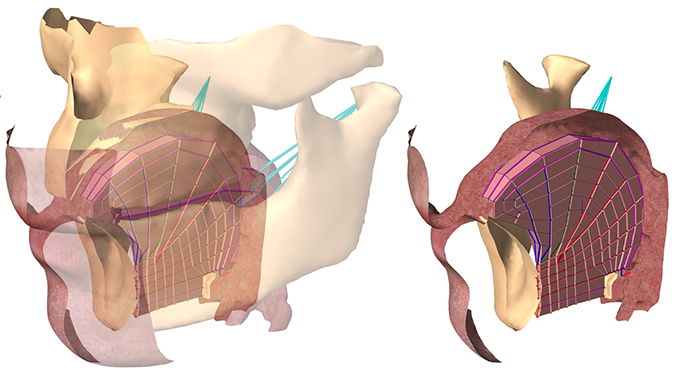
\includegraphics[width=5in]{images/AirwaySkinning}
 \caption{A skin mesh used to delimit the boundary of the human upper
airway, connected to various surrounding structures including
the palate, tongue, and jaw \cite{stavness2014unified}.}
\label{vocalTractSkin:fig}
\end{figure}

One application of skinning is to create a continuous skin surrounding
an underlying set of anatomical components. For example, for modeling
the human airway, a disparate set of models describing the tongue,
jaw, palate and pharynx can be connected together with a surface skin
to form a seamless airtight mesh (Figure \ref{vocalTractSkin:fig}), as
described in \cite{stavness2014unified}. This then provides a uniform
boundary for handling air or fluid interactions associated with tasks
such as speech or swallowing.

ArtiSynth provides support for ``skinning'' a mesh over an underlying
set of {\it master bodies}, consisting of rigid bodies and/or FEM
models, such that the mesh vertices deform in response to changes in
the position, orientation and shape of the master bodies.

\section{Implementation}
\label{skinningImplementation:sec}

This section describes the technical details of the ArtiSynth skinning
mechanism. A skin mesh is implemented using a
\javaclass[artisynth.core.femmodels]{SkinMeshBody}, which contains a
base mesh and references to a set of underlying dynamic {\it master
bodies}.  A master body can be either a
\javaclass[artisynth.core.mechmodels]{Frame} (of which
\javaclass[artisynth.core.mechmodels]{RigidBody} is a subclass), or a
\javaclass[artisynth.core.femmodels]{FemModel3d}. The positions of the
mesh vertices (along with markers and other points that can be
attached to the skin mesh) are determined by a weighted sum of
influences from each of the $m$ master bodies, such that as the latter
move and/or deform, the vertices and attached points deform as
well. More precisely, for each master body
$k, k \in \{0, \ldots, m-1\}$, let $w_k$ be the weighting factor and
$f_k(\q_k)$ the {\it connection function} that describes the
contribution of body $k$ to the position of the vertices (or attached
points) as a function of its generalized coordinates $\q_k$. Then if
the position of a vertex (or attached point) is denoted by $\p$ and
its initial (or {\it base}) position is $\p_0$, we have
%
\begin{equation}
\p = \sum_{k=0}^{m-1} w_k f_k (\q_k) + w_m \p_0.
\label{vertexpos:eqn}
\end{equation}
%
The weight $w_m$ in the last term is known as the {\it base weight}
and describes an optional contribution from the base position $\p_0$.
Usually $w_m = 0$, unless the vertex is not connected to {\tt any}
master bodies, in which case $w_m = 1$, so that the vertex is anchored
to its initial position.

In general, connection weights $w_k$ are computed based on the
distances $d_k$ between the vertex (or attached point) and
each master body $k$. More details on this are given in Sections
\ref{creatingSkinnedMesh:sec} and \ref{skinWeighting:sec}.

For {\tt Frame} master bodies, the connection function is one
associated with various rigid body skinning techniques known in the
literature. These include linear, linear dual quaternion, and
iterative dual quaternion skinning. Which technique is used is
determined by the {\sf frameBlending} property of the {\tt
SkinMeshBody}, which can be queried or set in code using the methods
%
\begin{lstlisting}[]
  FrameBlending getFrameBlending()

  void setFrameBlending (FrameBlending blending)
\end{lstlisting}
%
where \javaclassAlt{artisynth.core.femmodels.SkinMeshBody\$FrameBlending}%
{FrameBlending}
is an enumerated type defined by {\tt SkinMeshBody} with the following
values:

\begin{description}

\item[LINEAR]\mbox{}

Linear blending, in which the connection function $f_k()$ implements a
standard rigid connection between the vertex and the frame
coordinates. Let the frame's generalized coordinates $\q_k$ be given
by the $3 \times 3$ rotation matrix $\R$ and translation vector $\p_F$
describing its pose, with its initial pose given by $\R_{0}$ and
$\p_{F0}$. The connection function $f_k()$ then takes the form
%
\begin{equation}
f_k (\R, \p_F) = \R \R_0^T ( \p_0 - \p_{F0}) + \p_F.
\end{equation}
%
Linear blending is faster than other blending techniques but is more
prone to pinching and creasing artifacts in the presence of large
rotations between frames.

\item[DUAL\_QUATERNION\_LINEAR]\mbox{}

Linear dual quaternion blending, which is more computationally
expensive but typically gives better results than linear blending, and
is described in detail as DLB in \cite{kavan2008geometric}. Let the
frame's generalized coordinates $\q_k$ be given by the dual-quaternion
$\hat\q_k$ (describing both rotation and translation), with the
initial pose given by the dual-quaternion $\hat\q_{k0}$.  Then define
the relative dual-quaternion $\tilde\q_k$ as
%
\begin{equation}
\tilde\q_k = 
\frac{\hat\q_k \hat\q_{k0}^{-1}}{\| \sum_j w_j \hat\q_j \hat\q_{j0}^{-1} \|},
\end{equation}
%
where the denominator is formed by summing over {\it all} master
bodies $j$ which are frames.  The connection function $f_k()$ is then
given by
%
\begin{equation}
\f_k (\hat\q_k) = \tilde\q_k \p_0 \tilde\q_k^{-1} - \p_0,
\end{equation}
%
where we note that a dual quaternion multiplied by a position vector
yields a position vector.

\item[DUAL\_QUATERNION\_ITERATIVE]\mbox{}

Dual quaternion iterative blending, which is a more complex dual
quaternion technique described in detail as DIB in
\cite{kavan2008geometric}. The connection function for iterative dual
quaternion blending involves an iterative process and is not
described here. It also does not conform to (\ref{vertexpos:eqn}),
because the connection functions $f_k()$ for the {\tt Frame} master
bodies do not combine linearly. Instead, if there
are $r$ {\tt Frame} master bodies, there is a {\it single}
connection function
%
\begin{equation}
f (w_0, \ldots, w_{r-1}, \hat\q_0, \ldots, \hat\q_{r-1})
\end{equation}
%
that determines the connection for {\it all} of them, given their
weighting factors $w_j$ and generalized coordinates $\hat\q_j$.
Iterative blending relies on two parameters: a blend tolerance, and a
maximum number of blend steps, both of which are controlled by the
SkinMeshBody properties {\sf DQBlendTolerance} and {\sf
DQMaxBlendSteps}, which have default values of $1^{-8}$ and $3$.

\begin{sideblock}
Iterative dual quaternion blending is not completely supported in
ArtiSynth. In particular, because of its complexity, the associated
force and velocity mappings are computed using the simpler
computations employed for linear dual quaternion blending.  For the
examples shown in this chapter, iterative dual quaternion gives
results that are quite close to those of linear dual quaternion
blending.
\end{sideblock}

\end{description}

For FEM master bodies, the connection works by tying each vertex (or
attached point) to a specific FEM element using a fixed-length offset
vector $\d$ that rotates in conjunction with the element. This is
illustrated in Figure \ref{elementSkinning:fig} for the case of a
single FEM master body. Starting with the initial vertex position
$\p_0$, we find the nearest point $\p_{e0}$ on the nearest FEM
element, along with the offset vector $\d_0 \equiv \p_0 -
\p_{e0}$. The point $\p_{e0}$ can be expressed as the weighted
sum of the initial element nodal positions $\x_{j0}$,
%
\begin{equation}
\p_{e0} = \sum_{j=0}^{n-1} \alpha_j \x_{j0},
\end{equation}
%
where $n$ is the number of nodes and $\alpha_j$ represent the
(constant) nodal coordinates. As the element moves and deforms, the
element point $\p_e$ moves with the nodal positions $\x_j$ according
to the same relationship, while the offset vector $\d$ rotates
according to $\d = \R_E d_0$, where $\R_E$ is the rotation of the
element's coordinate frame $E$ with respect to its initial
orientation.  The connection function $f_k()$ then takes the form
%
\begin{equation}
f_k (\x_0, \ldots, \x_{n-1}) =
\sum_{j=0}^{n-1} \alpha_j \x_j + \R_E d_0.
\label{pelement:eqn}
\end{equation}
%
$\R_E$ is determined by computing a polar decomposition $\F = \R_E \P$
on the deformation gradient $\F$ at the element's center. We note that
the displacement $\d$ is only rotated and so the distance $\|\d\| =
\|\d_0\|$ of the vertex from the element remains constant. If the
vertex is initially on or inside the element, then $\d_0 = 0$ and
(\ref{pelement:eqn}) takes the form of a standard point/element
attachment as described in \ref{elementAttachment:sec}.

\begin{figure}[ht]
\begin{center}
 \includegraphics[width=3.5in]{images/elementSkinning}
\end{center}
\caption{Illustration of FEM skinning, showing how a position $\p$ is
tied to an FEM element.  Given the initial position $\p_0$, we find
the nearest point $\p_{e0}$ on the element, along with the offset
vector $\d_0 = \p_0 - \p_{e0}$ (left).  As the element moves and
deforms, the updated position is obtained from $\p = \p_e + \d$, where $\p_e$
deforms with the element, and $\d$ rotates in tandem with its
coordinate frame $E$.}
\label{elementSkinning:fig}
\end{figure}

\begin{sideblock}
While it is sometimes possible to determine weights $\alpha_j$ that
control a vertex position {\it outside} an element, without the need
for an offset vector $\d$, the resulting vertex positions tend to be
very sensitive to element distortions, particularly when the vertex is
located at some distance. Keeping the element-vertex distance constant
via an offset vector usually results in more plausible skinning
behavior.
\end{sideblock}

\section{Creating a skin mesh}
\label{creatingSkinnedMesh:sec}

As mentioned above, skin meshes within ArtiSynth are implemented
using the \javaclass[artisynth.core.femmodels]{SkinMeshBody}
component. Applications typically create a skin mesh in code
according to the following steps:

\begin{enumerate}

\item Create an instance of {\tt SkinMeshBody} and assign
its underlying mesh, usually within the constructor;

\item Add references to the required master bodies;

\item Compute the master body connections

\end{enumerate}

This is illustrated by the following example:
%
\begin{lstlisting}[]
  MechModel mech;
  PolygonalMesh mesh;

  // ... initialize mesh ...

  // create the body with an underlying mesh:
  SkinMeshBody skinMesh = new SkinMeshBody(mesh);
 
  // add references to the master bodies:
  skinMesh.addMasterBody (rigidBody1);
  skinMesh.addMasterBody (rigidBody2);
  skinMesh.addMasterBody (femModel1);
 
  // compute the weighted connections for each vertex:
  skinMesh.computeAllVertexConnections();

  // add to the MechModel
  mech.addMeshBody (skinMesh)
\end{lstlisting}
%
Master body references are added using
\javamethod[artisynth.core.femmodels.SkinMeshBody]{addMasterBody()}.
When all the master bodies have been added, the method\\
\javamethod[artisynth.core.femmodels.SkinMeshBody]{computeAllVertexConnections()}
computes the weighted connections to each vertex.  The connection
weights $w_k$ for each vertex are determined by a {\it weighting
function}, based on the distances $d_k$ between the vertex and each
master body. The default weighting function is {\it inverse-square
weighting}, which first computes a set of raw weights $w_k^*$
according to
%
\begin{equation}
w_k^* = \frac{d_\text{min}^2}{d_k^2},
\label{inverseSquareWeights:eqn}
\end{equation}
%
where $d_\text{min} \equiv \min( d_j)$ is the minimum master body distance,
and then normalizes these to determine $w_k$:
%
\begin{equation}
w_k = \frac{w^*_k}{\sum_j w^*_j}.
\label{normalizeWeights:eqn}
\end{equation}
%
Other weighting functions can be specified, as described in Section
\ref{skinWeighting:sec}.

{\tt SkinMeshBody} provides the following set of methods to set and
query its master body configuration:
%
\begin{lstlisting}[]
  void addMasterBody (ModelComponent body)    // add a master body
  int numMasterBodies()                       // query number of master bodies
  boolean hasMasterBody (ModelComponent body) // query master body presence
  ModelComponent getMasterBody (int idx)      // get a master body by index

  RigidTransform3d getBasePose (Frame frame)  // query base pose for frame
  void setBasePose (Frame frame, RigidTransform3d T) // set base pose for frame
\end{lstlisting}
%
When a {\tt Frame} master body is added using {\tt addMasterBody()},
its initial, or {\it base}, pose (corresponding to $\R_0$ and
$\p_{F0}$ in Section \ref{skinningImplementation:sec}) is set from its
current pose.  If necessary, applications can later query and reset
the base pose using the methods {\tt getBasePose()} and {\tt
setBasePose()}.

Internally, each vertex is connected to the master bodies by a
\javaclass[artisynth.core.femmodels]{PointSkinAttachment}, which
contains a list
of\\ \javaclass[artisynth.core.femmodels]{PointSkinAttachment\$SkinConnection}
components describing each master connection. Applications can obtain
the {\tt PointSkinAttachment} for each vertex using the method
%
\begin{lstlisting}[]
  PointSkinAttachment getVertexAttachment (int vidx)
\end{lstlisting}
%
where {\tt vidx} is the vertex index, which must be in the range 0 to
{\tt numv}-1, with {\tt numv} the number of vertices as returned by
{\tt numVertices()}.  Methods also exist to query and set each
vertex's base (i.e., initial) position $\p_0$:
%
\begin{lstlisting}[]
  Point3d getVertexBasePosition (int vidx)

  void setVertexBasePosition (int vidx, Point3d pos)
\end{lstlisting}
%

\subsection{Example: skinning over rigid bodies}

\begin{figure}[t]
\begin{center}
\iflatexml
 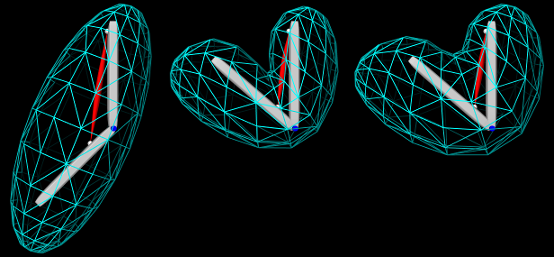
\includegraphics[]{images/RigidBodySkinningAll}
\else
 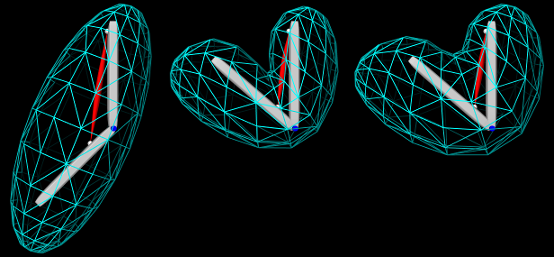
\includegraphics[width=6in]{images/RigidBodySkinningAll}
\fi
\end{center}
\caption{RigidBodySkinning model loaded into ArtiSynth (left), then
run with excitation set to 0.7 (middle). The right image shows the
result of changing the {\sf frameBlending} property from {\tt LINEAR}
to {\tt DUAL\_QUATERNION\_LINEAR}}.
\label{RigidBodySkinning:fig}
\end{figure}

An example of skinning a mesh over two rigid bodies is given by {\tt
artisynth.demos.tutorial.RigidBodySkinning}.  It consists of a {\tt
SkinMeshBody} placed around two rigid bodies connected by a hinge
joint to form a toy ``arm'', with a
\javaclass[artisynth.core.mechmodels]{Muscle} added to move the lower
body with respect to the upper.  
The code for the {\tt build()} method is given below:
\lstset{numbers=left}
\iflatexml
%% Hack: latexml lstinputlisting doesn't handle firstline correctly 
  \lstset{firstnumber={-35}}
  \lstinputlisting[firstline=1,lastline=68]{../../src/artisynth/demos/tutorial/RigidBodySkinning.java}
  \lstset{firstnumber={1}}
\else
  \lstinputlisting[firstline=37,lastline=104]{../../src/artisynth/demos/tutorial/RigidBodySkinning.java}
\fi
\lstset{numbers=none}

A {\tt MechModel} is created in the usual way (lines 2-7).  To this is
added a very simple toy ``arm'' consisting of an upper and lower body
connected by a hinge joint (lines 9-27), with a simple
point-to-point muscle attached between frame markers on the upper and
lower bodies to provide a means of moving the arm (lines 29-36).
Creation of the arm bodies uses an {\tt addBody()} method which is not
shown.

The mesh to be skinned is an ellipsoid, created using the
\javaclass[artisynth.core.femmodels]{FemFactory} method {\tt createSphere()}
to produce a spherical mesh which is then scaled and repositioned
(lines 38-43). The skin body itself is then created around this mesh,
with the upper and lower bodies assigned as master bodies and the
connections computed using {\tt computeAllVertexConnections()} (lines
45-50).

A control panel is added to allow control over the muscle's {\sf
excitation} as well as the skin body's {\sf frameBlending} property
(lines 52-56). Finally, render properties are set (lines 58-67): the
skin mesh is made transparent by setting its {\sf faceStyle} and
{\sf drawEdges} properties to {\tt NONE} and {\tt true}, respectively,
with cyan colored edges; the muscle is rendered as a red spindle; the
joint is drawn as a blue cylinder and the bodies are colored light
gray.

To run this example in ArtiSynth, select {\sf All demos > tutorial >
RigidBodySkinning} from the {\sf Models} menu. The model should load
and initially appear as in Figure \ref{RigidBodySkinning:fig}
(left). When running the simulation, the arm can be flexed by
adjusting the muscle {\sf excitation} property in the control panel,
causing the skin mesh to deform (Figure
\ref{RigidBodySkinning:fig}, middle). Changing the
{\sf frameBlending} property from its default value of {\tt LINEAR} to
{\tt DUAL\_QUATERNION\_LINEAR} causes the mesh deformation to become
fatter and less prone to creasing (Figure
\ref{RigidBodySkinning:fig}, right).

\section{Computing weights}
\label{skinWeighting:sec}

As described above, the default method for computing skin connection
weights is inverse-square weighting (equations \ref{inverseSquareWeights:eqn})
and \ref{normalizeWeights:eqn}). However, applications can specify
alternatives to this. The method
%
\begin{lstlisting}[]
  void setGaussianWeighting (double sigma)
\end{lstlisting}
%
causes weights to be computed according to a {\it Gaussian weighting}
scheme, with {\tt sigma} specifying the standard deviation $\sigma$.
Raw weights $w^*_k$ are then computed according to
%
\begin{equation*}
w_i = \text{exp} \left( -\frac{(d_k - d_\text{min})^2}{2 \sigma^2} \right),
\end{equation*}
%
and then normalized to form $w_k$.

The method
%
\begin{lstlisting}[]
  void setInverseSquareWeighting()
\end{lstlisting}
%
reverts the weighting function back to inverse-square weighting.

It is also possible to specify a custom weighting function
by implementing a subclass of 
\javaclass[artisynth.core.femmodels]{SkinWeightingFunction}.
Subclasses must implement the function
%
\begin{lstlisting}[]
  void computeWeights (
      double[] weights, Point3d pos, NearestPoint[] nearestPnts);
\end{lstlisting}
%
in which the weights for each master body are computed and returned in
{\tt weights}. {\tt pos} gives the initial position of the vertex (or
attached point) being skinning, while {\tt nearestPnts} provides
information about the distance from {\tt pos} to each of the master
bodies, using an array of
\javaclass[artisynth.core.femmodels]{SkinMeshBody\$NearestPoint}
objects:
%
\begin{lstlisting}[]
  class NearestPoint {
     public Point3d nearPoint;   // nearest point on the body
     public double distance;     // distance to the body
     public ModelComponent body; // master body (either Frame or FemModel3d)
  }
\end{lstlisting}
%

Once an instance of {\tt SkinWeightingFunction} has been created,
it can be set as the skin mesh weighting function by calling
%
\begin{lstlisting}[]
  void setWeightingFunction (SkinWeightingFunction fxn)
\end{lstlisting}
%
Subsequent calls to {\tt computeAllVertexConnections()}, or the {\tt
addMarker} or {\tt computeAttachment} methods described in Section
\ref{markersAndAttachments:sec}, will then employ the specified
weighting.

As an example, imagine an application wishes to compute weights
according to an inverse-cubic weighting function, such that
to
%
\begin{equation*}
w_k^* = \frac{d_\text{min}^3}{d_k^3}.
\end{equation*}
%
A subclass of {\tt SkinWeightingFunction} implementing this
could then be defined as
%
\begin{lstlisting}[]
class MyWeighting extends SkinWeightingFunction {
      
   // implements inverse-cubic weighting
   public void computeWeights (
      double[] weights, Point3d pos, NearestPoint[] nearestPnts) {

      // find minimum distance to all the master bodies
      double dmin = Double.POSITIVE_INFINITY;
      for (int i=0; i<nearestPnts.length; i++) {
         if (nearestPnts[i].distance < dmin) {
            dmin = nearestPnts[i].distance;
         }
      }
      double sumw = 0; // sum of all weights (for normalizing)
      // compute raw weights:
      for (int i=0; i<nearestPnts.length; i++) {
         double d = nearestPnts[i].distance;
         double w;
         if (d == dmin) {
            w = 1;  // handles case where dmin = d = 0
         }
         else {
            w = dmin*dmin*dmin/(d*d*d);
         }
         weights[i] = w;
         sumw += w;
      }
      // normalize the weights:
      for (int i=0; i<nearestPnts.length; i++) {
         weights[i] /= sumw;
      }
   }
}
\end{lstlisting}
and then set as the weighting function using the code fragment:
%
\begin{lstlisting}[]
   SkinMeshBody skinMesh;
   // ...
   skinMesh.setWeightingFunction (new MyWeighting());
\end{lstlisting}
%

The current weighting function for a skin mesh can be
queried using
%
\begin{lstlisting}[]
   SkinWeightingFunction getWeightingFunction()
\end{lstlisting}
%
The inverse-square and Gaussian weighting methods described above are
implemented using the system-provided {\tt SkinWeightingFunction}
subclasses
\javaclass[artisynth.core.femmodels]{InverseSquareWeighting} and
\javaclass[artisynth.core.femmodels]{GaussianWeighting}, respectively.

\subsection{Setting weights explicitly}

As an alternative to the weighting function, applications can also
create connections to vertices or points in which the weights are
explicitly specified. This allows for situations in which a weighting
function is unable to properly specify all the weights correctly.

When a mesh is initially added to a skin body, via either the
constructor
\javamethodAlt{artisynth.core.femmodels.SkinMeshBody.SkinMeshBody(MeshBase)}%
{SkinMeshBody(mesh)},
or by a call to
\javamethodAlt{artisynth.core.femmodels.SkinMeshBody.setMesh(MeshBase)}%
{setMesh(mesh)},
all master body connections are cleared and the vertex position is
``fixed'' to its initial position, also known as its {\it base
position}. After the master bodies have been added, vertex connections
can be created by calling
\javamethod[artisynth.core.femmodels.SkinMeshBody]{computeAllVertexConnections()},
as described above. However, connections can also be created on a
per-vertex basis, using the method
%
\begin{lstlisting}[]
  void computeVertexConnections (int vidx, VectorNd weights)
\end{lstlisting}
%
where {\tt vidx} is the index of the desired vertex and {\tt weights}
is an optional argument which if non-{\tt null} explicitly specifies
the connection weights. A sketch example of how this can be used is
given in the following code fragment:
%
\begin{lstlisting}[]
   VectorNd weights = new VectorNd (skinMesh.numMasterBodies());
   // compute connections for each vertex
   for (int i=0; i<skinMesh.numVertices(); i++) {
      // ... compute connections weights as required ...
      skinMesh.computeVertexConnections (i, weights);
   }
\end{lstlisting}
%
For comparison, it should be noted that the code fragment
\begin{lstlisting}[]
   for (int i=0; i<skinMesh.numVertices(); i++) {
      skinMesh.computeVertexConnections (i, null);
   }
\end{lstlisting}
in which weights are {\it not} explicitly specified, is
is equivalent to calling {\tt computeAllVertexConnections()}.

If necessary, after vertex connections have been computed, they can
also be cleared, using the method
%
\begin{lstlisting}[]
  void clearVertexConnections (int vidx)
\end{lstlisting}
%
This will disconnect the vertex with index {\tt vidx} from the master
bodies, and set its base weighting $w_m$ (equation
\ref{vertexpos:eqn}) to 1, so that it will remain fixed to its initial
position.

In some special cases, it may be desirable for an application to set
attachment base weights to some value other than 0 when connections
are present. Base weights for vertex attachments can be queried
and set using the methods
%
\begin{lstlisting}[]
   double getVertexBaseWeight (int vidx)

   void setVertexBaseWeight (int vidx, double weight, boolean normalize)
\end{lstlisting}
%
In the second method, the argument {\tt normalize}, if {\tt true},
causes the weights of the other connections to be scaled so that the
total weight sum remains the same. For skin markers and point attachments
(Section \ref{markersAndAttachments:sec}), base weights can be set
by calling the equivalent {\tt PointSkinAttachment} methods
%
\begin{lstlisting}[]
   double getBaseWeight ()

   void setBaseWeight (double weight, boolean normalize)
\end{lstlisting}
%
(If needed, the attachment for a skin marker can be obtained by
calling its {\tt getAttachment()} method.) In addition, base weights
can also be specified in the {\tt weights} argument to the method {\tt
computeVertexConnections(vidx,weights)}, as well as the methods {\tt
addMarker(name,pos,weights)} and {\tt
createPointAttachment(pnt,weights)} described in Section
\ref{markersAndAttachments:sec}. This is done by giving {\tt weights}
a size equal to $m+1$, where $m$ is the number of master bodies, and
specifying the base weight in the last location.

\section{Markers and point attachments}
\label{markersAndAttachments:sec}

In addition to controlling the positions of mesh vertices, a {\tt
SkinMeshBody} can also be used to control the positions of dynamic
point components, including markers and other points which can be
attached to the skin body. For both markers and attached points, any
applied forces are propagated back onto the skin body's master bodies,
using the principle of virtual work.  This allows skin bodies to be
fully incorporated into a dynamic model.

Markers and point attachments can be created even if the {\tt
SkinMeshBody} does not have a mesh, a fact that can be used in
situations where a mesh is unnecessary, such as when employing skinning
techniques for muscle wrapping (Section \ref{skinBasedWrapping:sec}).

\subsection{Markers}

Markers attached to a skin body are instances of
\javaclass[artisynth.core.femmodels]{SkinMarker}, and are contained in
the body's subcomponent list {\tt markers} (analogous to the {\tt
markers} list for FEM models). Markers can be created and maintained
using the following {\tt SkinMeshBody} methods:
%
\begin{lstlisting}[]
  // create markers:
  SkinMarker addMarker (Point3d pos)
  SkinMarker addMarker (String name, Point3d pos)
  SkinMarker addMarker (
     String name, Point3d pos, VectorNd weights)

  // remove markers:
  boolean removeMarker (SkinMarker mkr)
  void clearMarkers();

  // access the marker list:
  PointList<SkinMarker> markers()
\end{lstlisting}
%
The {\tt addMarker} methods each create and return a {\tt SkinMarker}
which is added to the skin body's list of markers. The marker's
initial position is specified by {\tt pos}, while the second and third
methods also allow a name to be specified. Connections between the
marker and the master bodies are created in the same way as for mesh
vertices, with the connection weights either being determined by the
skin body's weighting function (as returned by
\javamethod[artisynth.core.femmodels.SkinMeshBody]{getWeightingFunction()}),
or explicitly specified by the argument {\tt weights} (third method).

Once created, markers can be removed individually or all together by
the {\tt removeMarker()} and {\tt clearMarkers()} methods. The entire
marker list can be accessed on a read-only basis by the method
{\tt markers()}.

\subsection{Point attachments}

In addition to markers, applications can also attach any regular
\javaclass[artisynth.core.mechmodels]{Point} component (including
particles and FEM nodes) to a skin body by using one of its
{\tt createPointAttachment} methods:
%
\begin{lstlisting}[]
  PointSkinAttachment createPointAttachment (Point pnt)
  PointSkinAttachment createPointAttachment (Point pnt, VectorNd weights)
\end{lstlisting}
%
Both of these create a
\javaclass[artisynth.core.femmodels]{PointSkinAttachment} that
connects the point {\tt pnt} to the master bodies in the same way as
for mesh vertices and markers, with the connection weights either
being determined by the skin body's weighting function or explicitly
specified by the argument {\tt weights} in the second method.

Once created, the point attachment must also be added to the
underlying {\tt MechModel}, as illustrated by the following code
fragment:
%
\begin{lstlisting}[]
  MechModel mech;
  SkinMeshBody skinBody;
  Point pnt;

  // ... initialize ...

  PointSkinAttacment a = skinBody.createPointAttachment(pnt);
  mech.addAttachment (a);
\end{lstlisting}
%

\subsection{Example: skinning rigid bodies and FEM models}

\begin{figure}[t]
\begin{center}
\iflatexml
 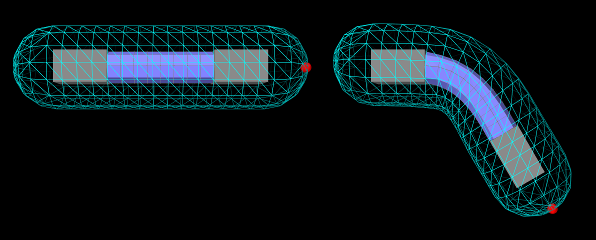
\includegraphics[]{images/AllBodySkinning}
\else
 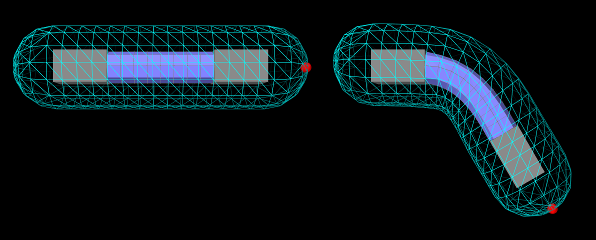
\includegraphics[width=6in]{images/AllBodySkinning}
\fi
\end{center}
\caption{AllBodySkinning model as first loaded into ArtiSynth (left),
and after the simulation is run and the model has fallen under gravity
(right). The skin mesh is rendered in cyan using only its edges.}
\label{AllBodySkinning:fig}
\end{figure}

An example of skinning a mesh over both rigid bodies and FEM models is
given by the demo model\\
{\tt artisynth.demos.tutorial.AllBodySkinning}.  It consists
of a skin mesh placed around a tubular FEM model
connected to rigid bodies connected at each end, and a
marker attached to the mesh tip.
The code for the {\tt build()} method is given below:
\lstset{numbers=left} \iflatexml
%% Hack: latexml lstinputlisting doesn't handle firstline correctly 
  \lstset{firstnumber={-27}}
  \lstinputlisting[firstline=1,lastline=65]{../../src/artisynth/demos/tutorial/AllBodySkinning.java}
  \lstset{firstnumber={1}}
\else
  \lstinputlisting[firstline=29,lastline=93]{../../src/artisynth/demos/tutorial/AllBodySkinning.java}
\fi
\lstset{numbers=none}

A {\tt MechModel} is first created and length and density parameters
are defined (lines 2-8). Then a tubular FEM model is created, by using
the \javaclass[artisynth.core.femmodels]{FemFactory} method {\tt
createHexTube()} and transforming the result by rotating it by 90
degrees about the $y$ axis (lines 10-14). Two rigid body blocks are
then created (lines 16-26) and attached to the ends of the FEM model
by finding and attaching the left and rightmost nodes (lines 28-24).
The model is anchored to ground by setting the left block to be
non-dynamic (line 21).

The mesh to be skinned is a rounded cylinder, created using the
\javaclass[maspack.geometry]{MeshFactory} method {\tt
createRoundedCylinder()} and rotating the result by 90 degrees about
the $y$ axis (lines 39-44). This is then used to create the skin body
itself, to which both rigid bodies and the FEM model are added as
master bodies and the vertex connections are computed using a call to
{\tt computeAllVertexConnections()} (lines 46-52). A marker is then
added to the tip of the skin body, using the {\tt addMarker()} method
(lines 54-56). Finally render properties are set (lines 58-64):
The mesh is made transparent by drawing only its edges in cyan; the
FEM model surface mesh is rendered in blue-gray, and the
tip marker is drawn as a red sphere.

To run this example in ArtiSynth, select {\sf All demos > tutorial >
AllBodySkinning} from the {\sf Models} menu. The model should load and
initially appear as in Figure \ref{AllBodySkinning:fig} (left). When
running the simulation, the FEM and the rightmost rigid body fall
under gravity, causing the skin mesh to deform. The pull tool
can then be used to move things around by applying forces to the
master bodies or the skin mesh itself.

\subsection{Mesh-based markers and attachments}

For the markers and point attachments described above, the connections
to the underlying master bodies are created in the same manner as
connections for individual mesh vertices. This means that the
resulting markers and attached points move {\it independently} of the
mesh vertices, as though they were vertices in their own right.

An advantage to this is that such markers and attachments can be
created even if the {\tt SkinMeshBody} does not even have a mesh, as
noted above. However, a disadvantage is that such markers will not
remain tightly connected to vertex-based features (such as the faces
of a \javaclass[maspack.geometry]{PolygonalMesh} or the line segments
of a \javaclass[maspack.geometry]{PolylineMesh}). For example,
consider a marker defined by
%
\begin{lstlisting}[]
  SkinMarker mkr = skinBody.addMarker (pos);
\end{lstlisting}
%
where {\tt pos} is a point that is initially located on a face of the
body's mesh. As the master bodies move and the mesh deforms, the
resulting marker may not remain strictly on the face. In many cases,
this may not be problematic or the deviation may be too small to
matter. However, {\it if} it is desirable for markers or point
attachments to be tightly bound to mesh features, they can instead be
created with the following methods:
%
\begin{lstlisting}[]
  // create mesh-based markers:
  SkinMarker addMeshMarker (Point3d pos)
  SkinMarker addMeshMarker (String name, Point3d pos)

  // create mesh-based attachments:
  PointSkinAttachment createPointMeshAttachment (Point pnt)
\end{lstlisting}
%
The requested position {\tt pos} will then be projected onto the
nearest mesh feature (e.g., a face for a {\tt PolygonalMesh} or a line
segment for a {\tt PolylineMesh}), and the resulting position $\p$
will be defined as a linear combination of the vertex positions
$\p_i$ for this feature,
%
\begin{equation}
\p = \sum_i \beta_i \p_i,
\end{equation}
%
where $\beta_i$ are the barycentric coordinates of $\p$ with respect
to the feature. The master body connections are then defined by the
same linear combination of the connections for each vertex.  When the
master bodies move, the marker or attached point will move with the
feature and remain in the same relative position.

Since {\tt SkinMeshBody} implements the interface
\javaclass[artisynth.core.mechmodels]{PointAttachable}, it
provides the general point attachment method
%
\begin{lstlisting}[]
  PointSkinAttachment createPointAttachment (Point pnt)
\end{lstlisting}
%
which allows it to be acted on by agents such as the ArtiSynth marker
tool (see the section ``Marker tool'' in the
\artisynthManual{uiguide}{ArtiSynth User Interface Guide}).  Whether
or not the resulting attachment is a regular attachment or mesh-based
is controlled by the skin body's {\sf attachPointsToMesh} property,
which can be adjusted in the GUI or in code using the property's
accessor methods:
%
\begin{lstlisting}[]
  boolean getAttachPointsToMesh()
  void setAttachPointsToMesh (boolean enable)
\end{lstlisting}
%
\section{Resolution and Limitations}

Skinning techniques do have limitations, which are common to all
methodologies.

\begin{figure}[t]
\begin{center}
\iflatexml
 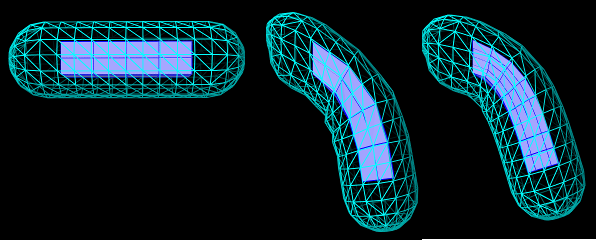
\includegraphics[]{images/FemSkinResAll}
\else
 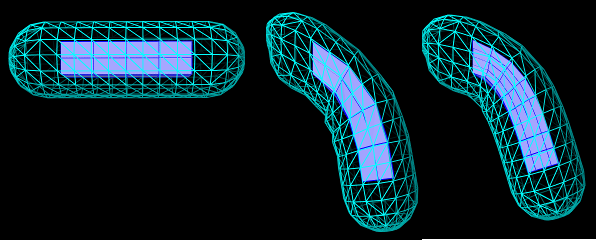
\includegraphics[width=6in]{images/FemSkinResAll}
\fi
\end{center}
\caption{A skin mesh enveloping a single FEM body whose
element resolution is lower than that of the mesh (left). When
the FEM undergoes a large deformation,
this disparity in resolution can cause artifacts
such as crimping, as seen on the underside of the mesh
in the middle image. Using an FEM model with a higher
resolution can mitigate this (right).}
\label{FemSkinResAll:fig}
\end{figure}

\begin{itemize}

\item The passive nature of the connection between skinned vertices
and the master bodies means that it can be easy for the skin mesh
to self intersect and/or fold and crease in ways that are not
physically realistic. These effects are often more pronounced when
mesh vertices are relatively far away from the master bodies, or in
places where the mesh undergoes a concave deformation. When the master
bodies include frames, these effects can sometimes be reduced by
setting the {\sf frameBlending} property to {\tt
DUAL\_QUATERNION\_LINEAR} instead of the default {\tt LINEAR}.

\item When the master bodies include FEM models which undergo large
deformations, crimping artifacts may arise if the skin mesh has a
higher resolution that the FEM model (Figure
\ref{FemSkinResAll:fig}). This is because each mesh vertex is
connected to the coordinate frame of a single FEM element, and for
reasons of computational efficiency the influence of these coordinate
frames is not blended as it is for frame-based master bodies.  If
crimping artifacts occur, one solution may be to adjust the mesh
and/or the FEM model so that their resolutions are more compatible
(Figure \ref{FemSkinResAll:fig}, right).

\end{itemize}

\section{Collisions}
\label{SkinCollisions:sec}

It is possible to make skin bodies collide with other ArtiSynth
bodies, such as {\tt RigidBody} and {\tt FemModel3d}, which implement
the \javaclass[artisynth.core.mechmodels]{Collidable} interface
(Chapter \ref{ContactAndCollision:sec}). {\tt SkinMeshBody} itself
implements \javaclass[artisynth.core.mechmodels]{CollidableBody}, and
is considered a deformable body, so that collisions can be activated
either by setting one of the default collision behaviors involving
deformable bodies, or by setting an explicit collision behavior
between it and another body. Self collisions involving {\tt
SkinMeshBody} are not currently supported.

As described in Section \ref{CollisionImplementation:sec}, collisions
work by computing the intersection between the meshes of the skin body
and other collidables. The vertices, faces, and (possibly) edges of
the resulting intersection region are then used to compute contact
constraints, which propagate the effect of the contact back onto the
collidable bodies' dynamic components. For a skin mesh, the dynamic
components are the Frame master bodies and the nodes of the FEM master
bodies.

Collisions involving {\tt SkinMeshBody} frequently suffer from the
problem of being overconstrained (Section
\ref{OverconstrainedContact:sec}), whereby the the number of contacts
exceeds the number of master body DOFs available to handle the
collision. This may occur if the skin body contains only rigid bodies,
or if the mesh resolution exceeds the resolution of the FEM master
bodies. Managing overconstrained collisions is discussed in Section
\ref{OverconstrainedContact:sec}, with the easiest method being
constraint reduction, which can be activated by setting to {\tt true}
the {\sf reduceConstraints} property for either the collision manager
{\it or} a specific
\javaclass[artisynth.core.mechmodels]{CollisionBehavior} involving the
skin body.

\begin{sideblock}
Caveats: The distance between the vertices of a skinned mesh and its
master bodies can sometimes cause odd or counter-intuitive collision
behavior. Collision handling may also be noticeably slower if {\sf
frameBlending} is set to {\tt DUAL\_QUATERNION\_LINEAR} or {\tt
DUAL\_QUATERNION\_ITERATIVE}. If any of the master bodies are FEM
models, collisions resulting in large friction forces may result in
unstable behavior.
\end{sideblock}

\subsection{Example: collision with a cylinder}

\begin{figure}[t]
\begin{center}
\iflatexml
 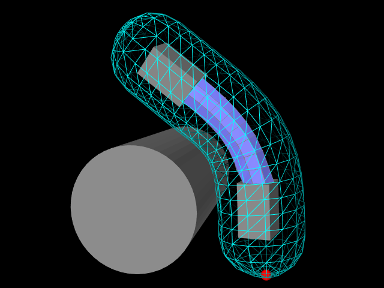
\includegraphics[]{images/SkinBodyCollide}
\else
 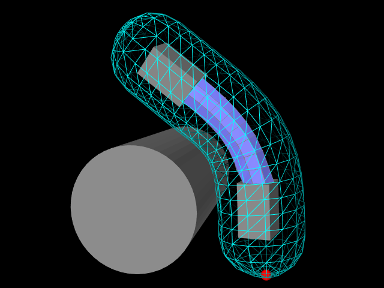
\includegraphics[width=3.5in]{images/SkinBodyCollide}
\fi
\end{center}
\caption{{\tt SkinBodyCollide} demo, showing a skin mesh colliding
with a cylinder about 0.6 seconds into the simulation.}
\label{SkinBodyCollide:fig}
\end{figure}

Collisions involving {\tt SkinMeshBody} are illustrated by the demo
model {\tt artisynth.demos.tutorial.SkinBodyCollide}, which extends
the demo {\tt AllBodySkinning} to add a cylinder with which the skin
body can collide. 
The code for the demo is given below:
\lstset{numbers=left} 
\lstinputlisting[]{../../src/artisynth/demos/tutorial/SkinBodyCollide.java}
\lstset{numbers=none}

The model subclasses {\tt AllBodySkinning}, using the superclass {\tt
build()} method within its own {\tt build{}} method to create the
original model (line 12). It then obtains references to the {\tt
MechModel}, {\tt SkinMeshBody}, and leftmost block, using their names
to find them in various component lists (lines 14-17).  (If the
original model had stored references to these components as accessible
member attributes, this step would not be needed.)

These component references are then used to make changes to the model:
the left block is made dynamic so that the skin mesh can fall freely
(line 21), a cylinder is created and added (lines 23-30), collisions
are enabled between the skin body and the cylinder (lines 32-34), and
the collision manager is asked to use constraint reduction to minimize
the chance of overconstrained contact (line 35).

To run this example in ArtiSynth, select {\sf All demos > tutorial >
SkinBodyCollide} from the {\sf Models} menu. When run,
the skin body should fall and collide with the cylinder
as shown in Figure \ref{SkinBodyCollide:fig}.

\section{Application to muscle wrapping}
\label{skinBasedWrapping:sec}

It is sometimes possible to use skinning as a computationally cheaper
way to implement muscle wrapping (Chapter
\ref{multipointSpringIntro:sec}).

Typically, the end points (i.e., origin and insertion points) of a
point-to-point muscle are attached to different bodies. As these
bodies move with respect to each other, the path of the muscle may
{\it wrap} around portions of these bodies and perhaps other
intermediate bodies as well. The wrapping mechanism of Chapter
\ref{multipointSpringIntro:sec} manages this by performing the
computations necessary to allow one or more {\it wrappable} segments
of a \javaclass[artisynth.core.mechmodels]{MultiPointSpring} to wrap
around a prescribed set of rigid bodies. However, if the induced path
deformation is not too great, it may be possible to achieve a similar
effect at much lower computational cost by simply ``skinning'' the via
points of the multipoint spring to the underlying rigid bodies.

The general approach involves:

\begin{enumerate}

\item Creating a \javaclass[artisynth.core.femmodels]{SkinMeshBody}
which references as master bodies the bodies containing the origin and
insertion points, and possibly other bodies as well;

\item Creating the wrapped muscle using a 
\javaclass[artisynth.core.mechmodels]{MultiPointSpring}
with via points that are attached to the skin body.
        
\end{enumerate}

It should be noted that for this application, the skin body does not
need to contain a mesh. Instead, ``skinning'' connections can be made
solely between the master bodies and the via points. An easy way to do
this is to simply use skin body markers as via points.  Another way is
to create the via points as separate particles, and then attach them
to the skin body using one of its {\tt createPointAttachment} methods.

\begin{sideblock}
It should also be noted that unlike with the wrapping methods of
Chapter \ref{multipointSpringIntro:sec}, skin-based wrapping can be
applied around FEM models as well as rigid bodies.
\end{sideblock}

\begin{sideblock}
Generally, we observe better wrapping behavior if the {\sf
frameBlending} property of the {\tt SkinMeshBody} is set to {\tt
DUAL\_QUATERNION\_LINEAR} instead of the default value of {\tt
LINEAR}.
\end{sideblock}

\subsection{Example: wrapping for a finger joint}

\begin{figure}[t]
\begin{center}
\iflatexml
 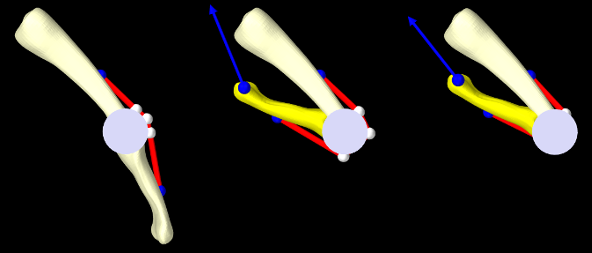
\includegraphics[]{images/PhalanxSkinWrapping}
\else
 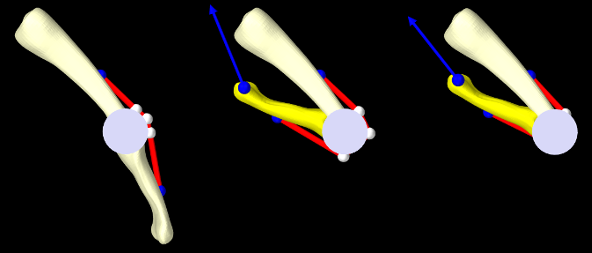
\includegraphics[width=6in]{images/PhalanxSkinWrapping}
\fi
\end{center}
\caption{PhalanxSkinWrapping model loaded into ArtiSynth and running
with no load on the distal bone (left). The pull tool is then
used to exert forces on the distal bone and pull it around the joint
(middle).  The viewer has been set to {\sf orthographic} projection to
enable better visualization of the wrapping behavior of the muscle via
points (shown in white). The results appear better when the
SkinMeshBody's {\sf frameBlending} property is set to {\tt
DUAL\_QUATERNION\_LINEAR} (middle) instead of {\tt LINEAR} (right).}
\label{PhalanxSkinWrapping:fig}
\end{figure}

An example of skinning-based muscle wrapping is given by {\tt
artisynth.demos.tutorial.PhalanxSkinWrapping}, which is identical to
the demo {\tt artisynth.demos.tutorial.PhalanxWrapping} except for
using skinning to achieve the wrapping effect. The portion of the
code which differs is shown below: \lstset{numbers=left} \iflatexml
%% Hack: latexml lstinputlisting doesn't handle firstline correctly
\lstset{firstnumber={-66}}
\lstinputlisting[firstline=1,lastline=41]{../../src/artisynth/demos/tutorial/PhalanxSkinWrapping.java}
\lstset{firstnumber={1}}
\else
\lstinputlisting[firstline=68,lastline=108]{../../src/artisynth/demos/tutorial/PhalanxSkinWrapping.java}
\fi
\lstset{numbers=none}

First, a {\tt SkinMeshBody} is created referencing the proximal and
distal bones as master bodies, with the {\sf frameBlending} property
set to {\tt DUAL\_QUATERNION\_LINEAR} (lines 1-6).  Next, we create a
set of three via points that will be attached to the skin body to
guide the muscle around the joint in lieu of making it actually wrap
around a cylinder (lines 7-9).

In the original {\tt PhalanxWrapping} demo, a
\javaclass[artisynth.core.mechmodels]{RigidCylinder} was used as a
muscle wrap surface. In this demo, we replace this with a simple
cylindrical mesh which has no dynamic function but allows us to
visualize the wrapping behavior of the via points (lines 11-18).  The
muscle itself is created using the three via points but with no
wrappable segments or bodies (lines 20-30).

A control panel is added to allow for the adjustment of the skin
body's {\sf frameBlending} property (lines 32-35). Finally, render
properties are set as for the original demo, only with the skin body
markers rendered as white spheres to make them more visible (lines
37-41).

To run this example in ArtiSynth, select {\sf All demos > tutorial >
PhalanxSkinWrapping} from the {\sf Models} menu. The model should load
and initially appear as in Figure \ref{PhalanxSkinWrapping:fig}
(left). The pull tool can then be used to move the distal joint
while simulating, to illustrate how well the via points ``wrap''
around the joint, using the cylindrical mesh as a visual reference
(Figure \ref{PhalanxSkinWrapping:fig}, middle).  Changing the {\sf
frameBlending} property to {\tt LINEAR} results in a less satisfactory
behavior (Figure \ref{PhalanxSkinWrapping:fig}, right).

\ifdefined\maindoc
\else
\end{document}
\fi
